\documentclass[12pt]{article}
\usepackage[utf8]{inputenc}

\newenvironment{sol}[1][Solution]{\begin{trivlist}\item[\hskip\labelsep {\bfseries #1:}]}{\end{trivlist}}
\usepackage[margin=1in]{geometry} 
\usepackage{amsmath,amsthm,amssymb}
\usepackage{minted}
\usemintedstyle{vs}
\usepackage{graphicx}
\graphicspath{{./images}}
\usepackage{ amssymb }

\title{CS7381 Project 3 \\ 
MIPS Assembly Code Programming Using MARS Tool – Additional Coding Assignment }

\author{
Name: Bingying Liang \\
ID: 48999397\\  
Distance}
\date{February 19 2023}

\begin{document}

\maketitle

For this exercise, you will write another MIPS assembly code program.   This time, you will create and run MIPS code for the following high-level language (HLL) code:\\
\centering \noindent C\texttt{++} Version
\begin{minted}
[frame=lines,fontsize=\footnotesize]{c++}
int j, k, n, x;
x = 1;
n = 4;
j = n;
// outer loop with j
do
{
    k = n;
    // inner loop with k
    do
    {
        x = x + 2 * j + 1;
        cout << x << " ";
        k--;
    } while (k > 0);
    j--;
} while (j > 0);
\end{minted}
\centering Java Version
\begin{minted}[frame=lines,fontsize=\footnotesize]{python}
x = 1
n = 4
j = n
# outer loop with j
while True:   
    k = n
    # inner loop with k
    while True:
        x = x + 2 * j + 1
        print(x, end=" ")
        k -= 1
        if (k == 0):
            break
    j -= 1
    if (j == 0):
        break
\end{minted}

\leftline{\textbf{Screen shot of the MARS console}}
    \begin{center}
        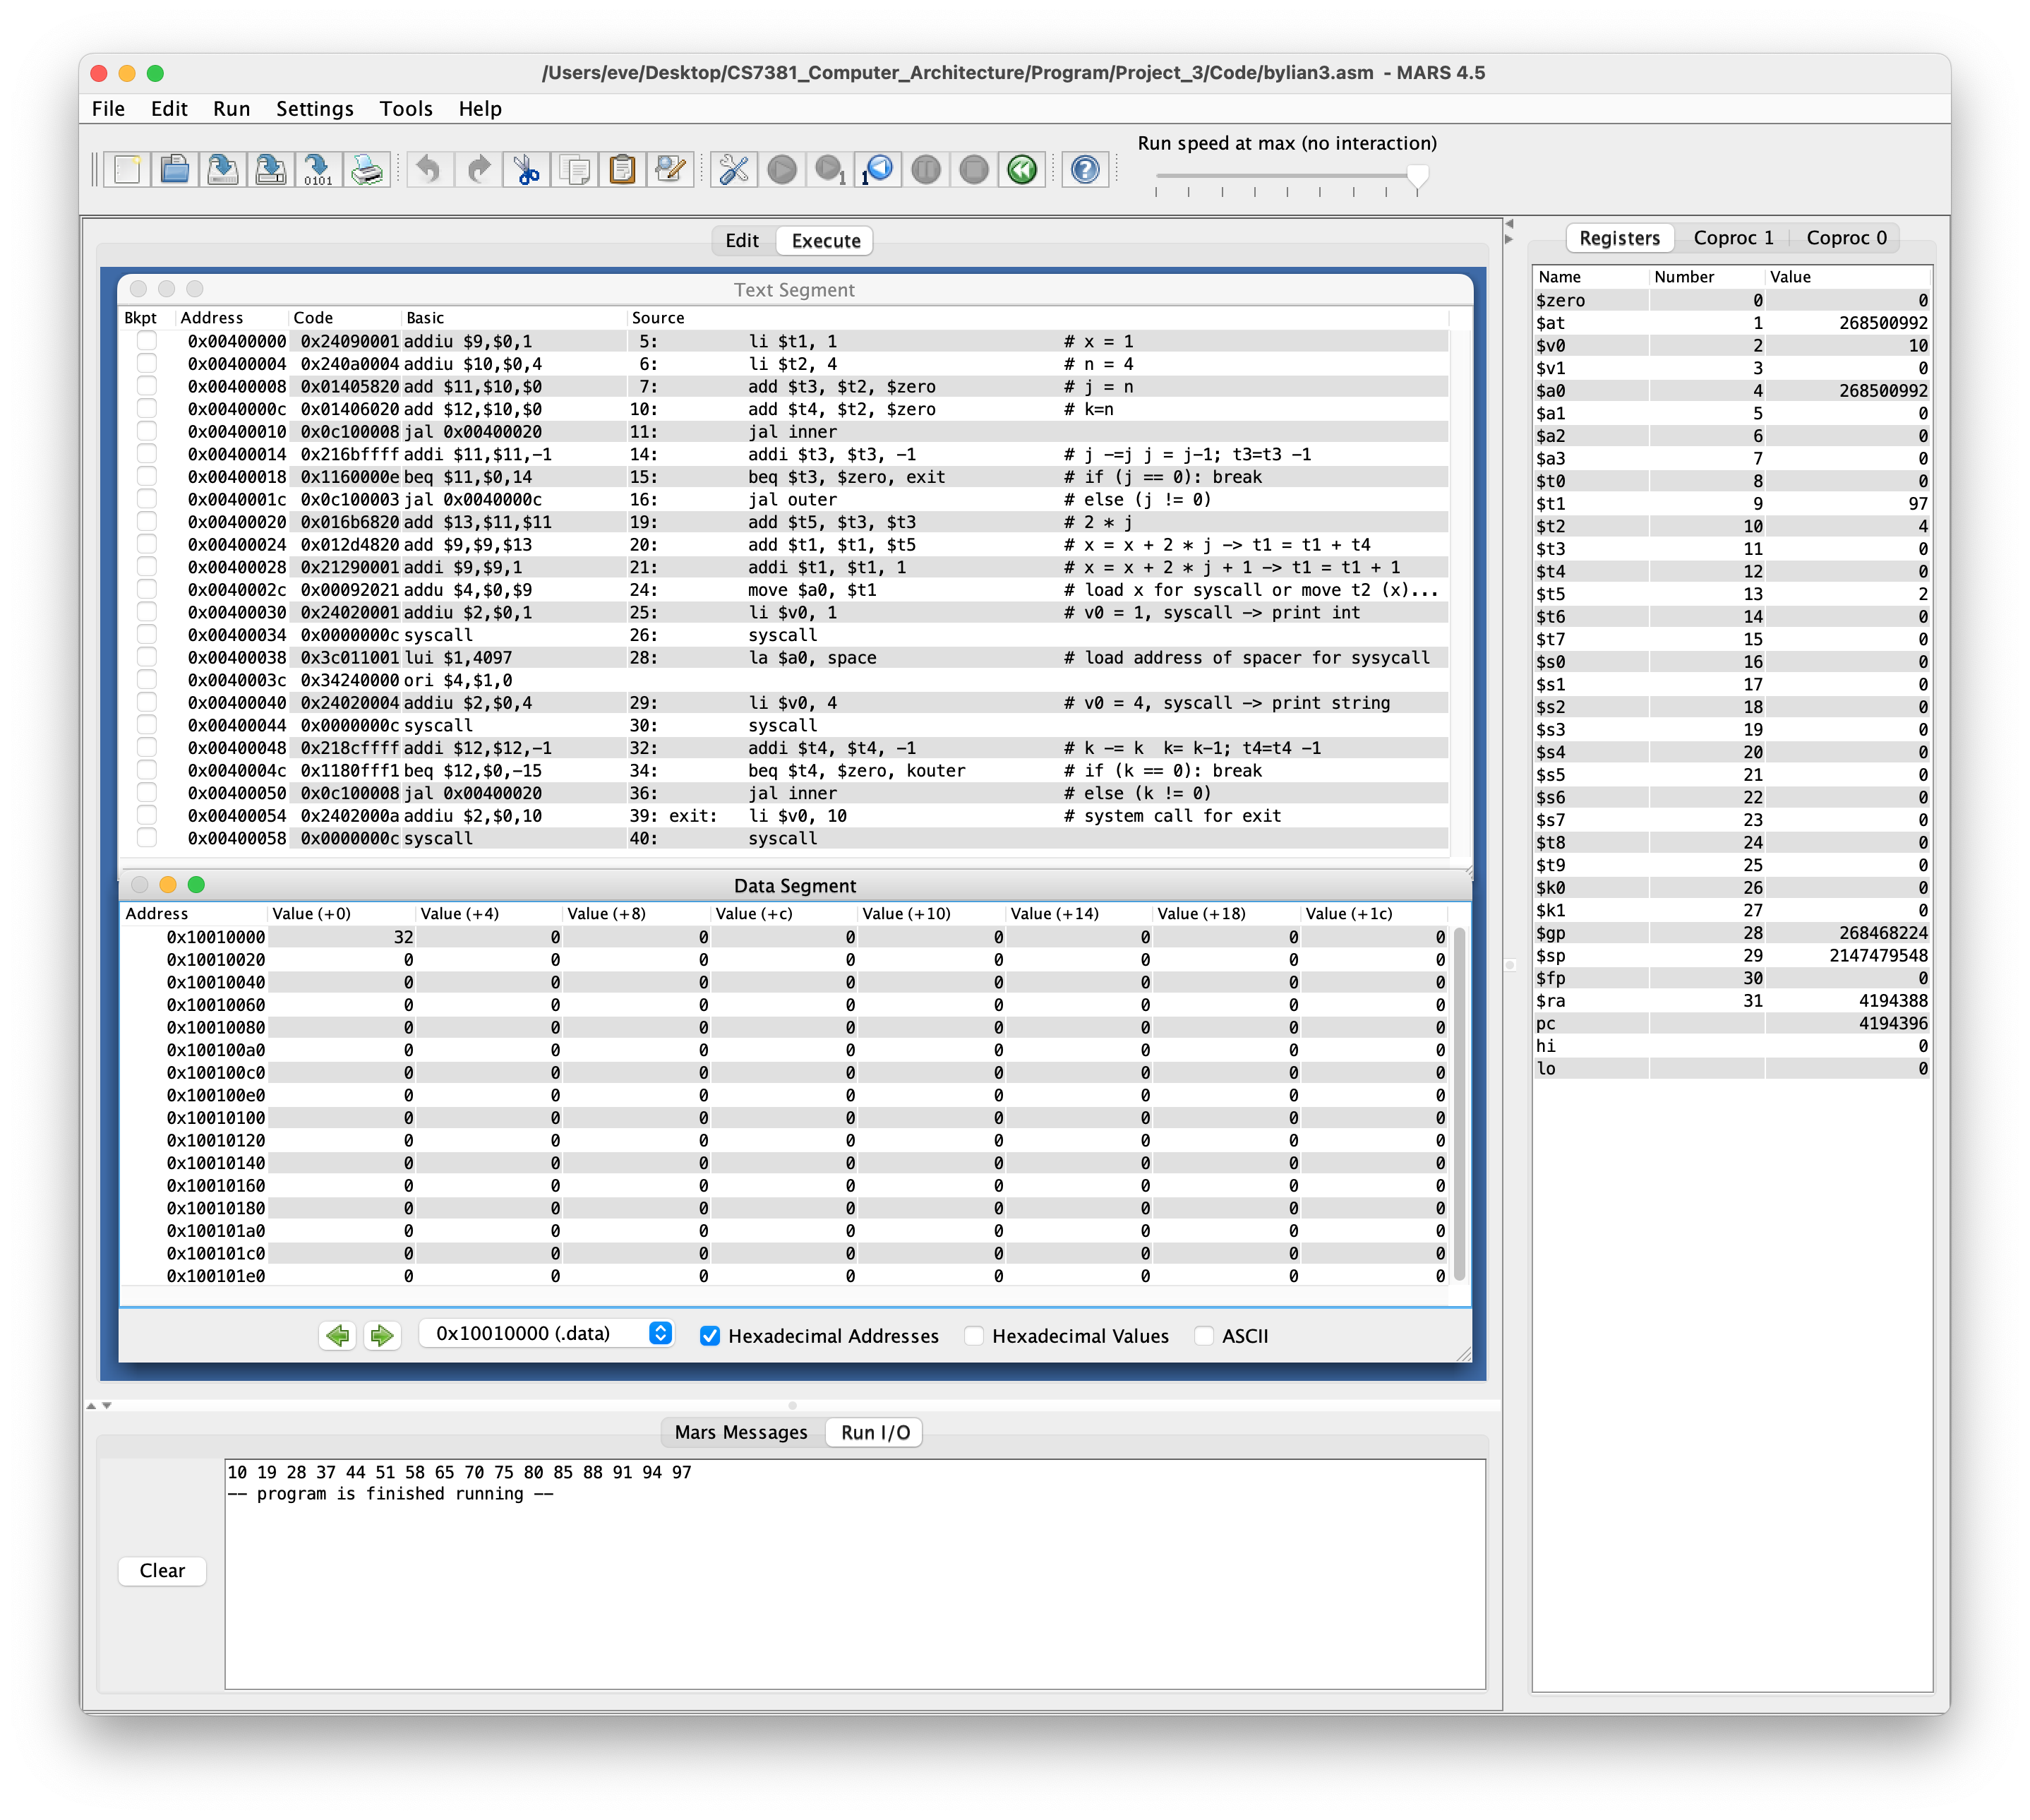
\includegraphics[width=1.1\textwidth]{p1.png} 
        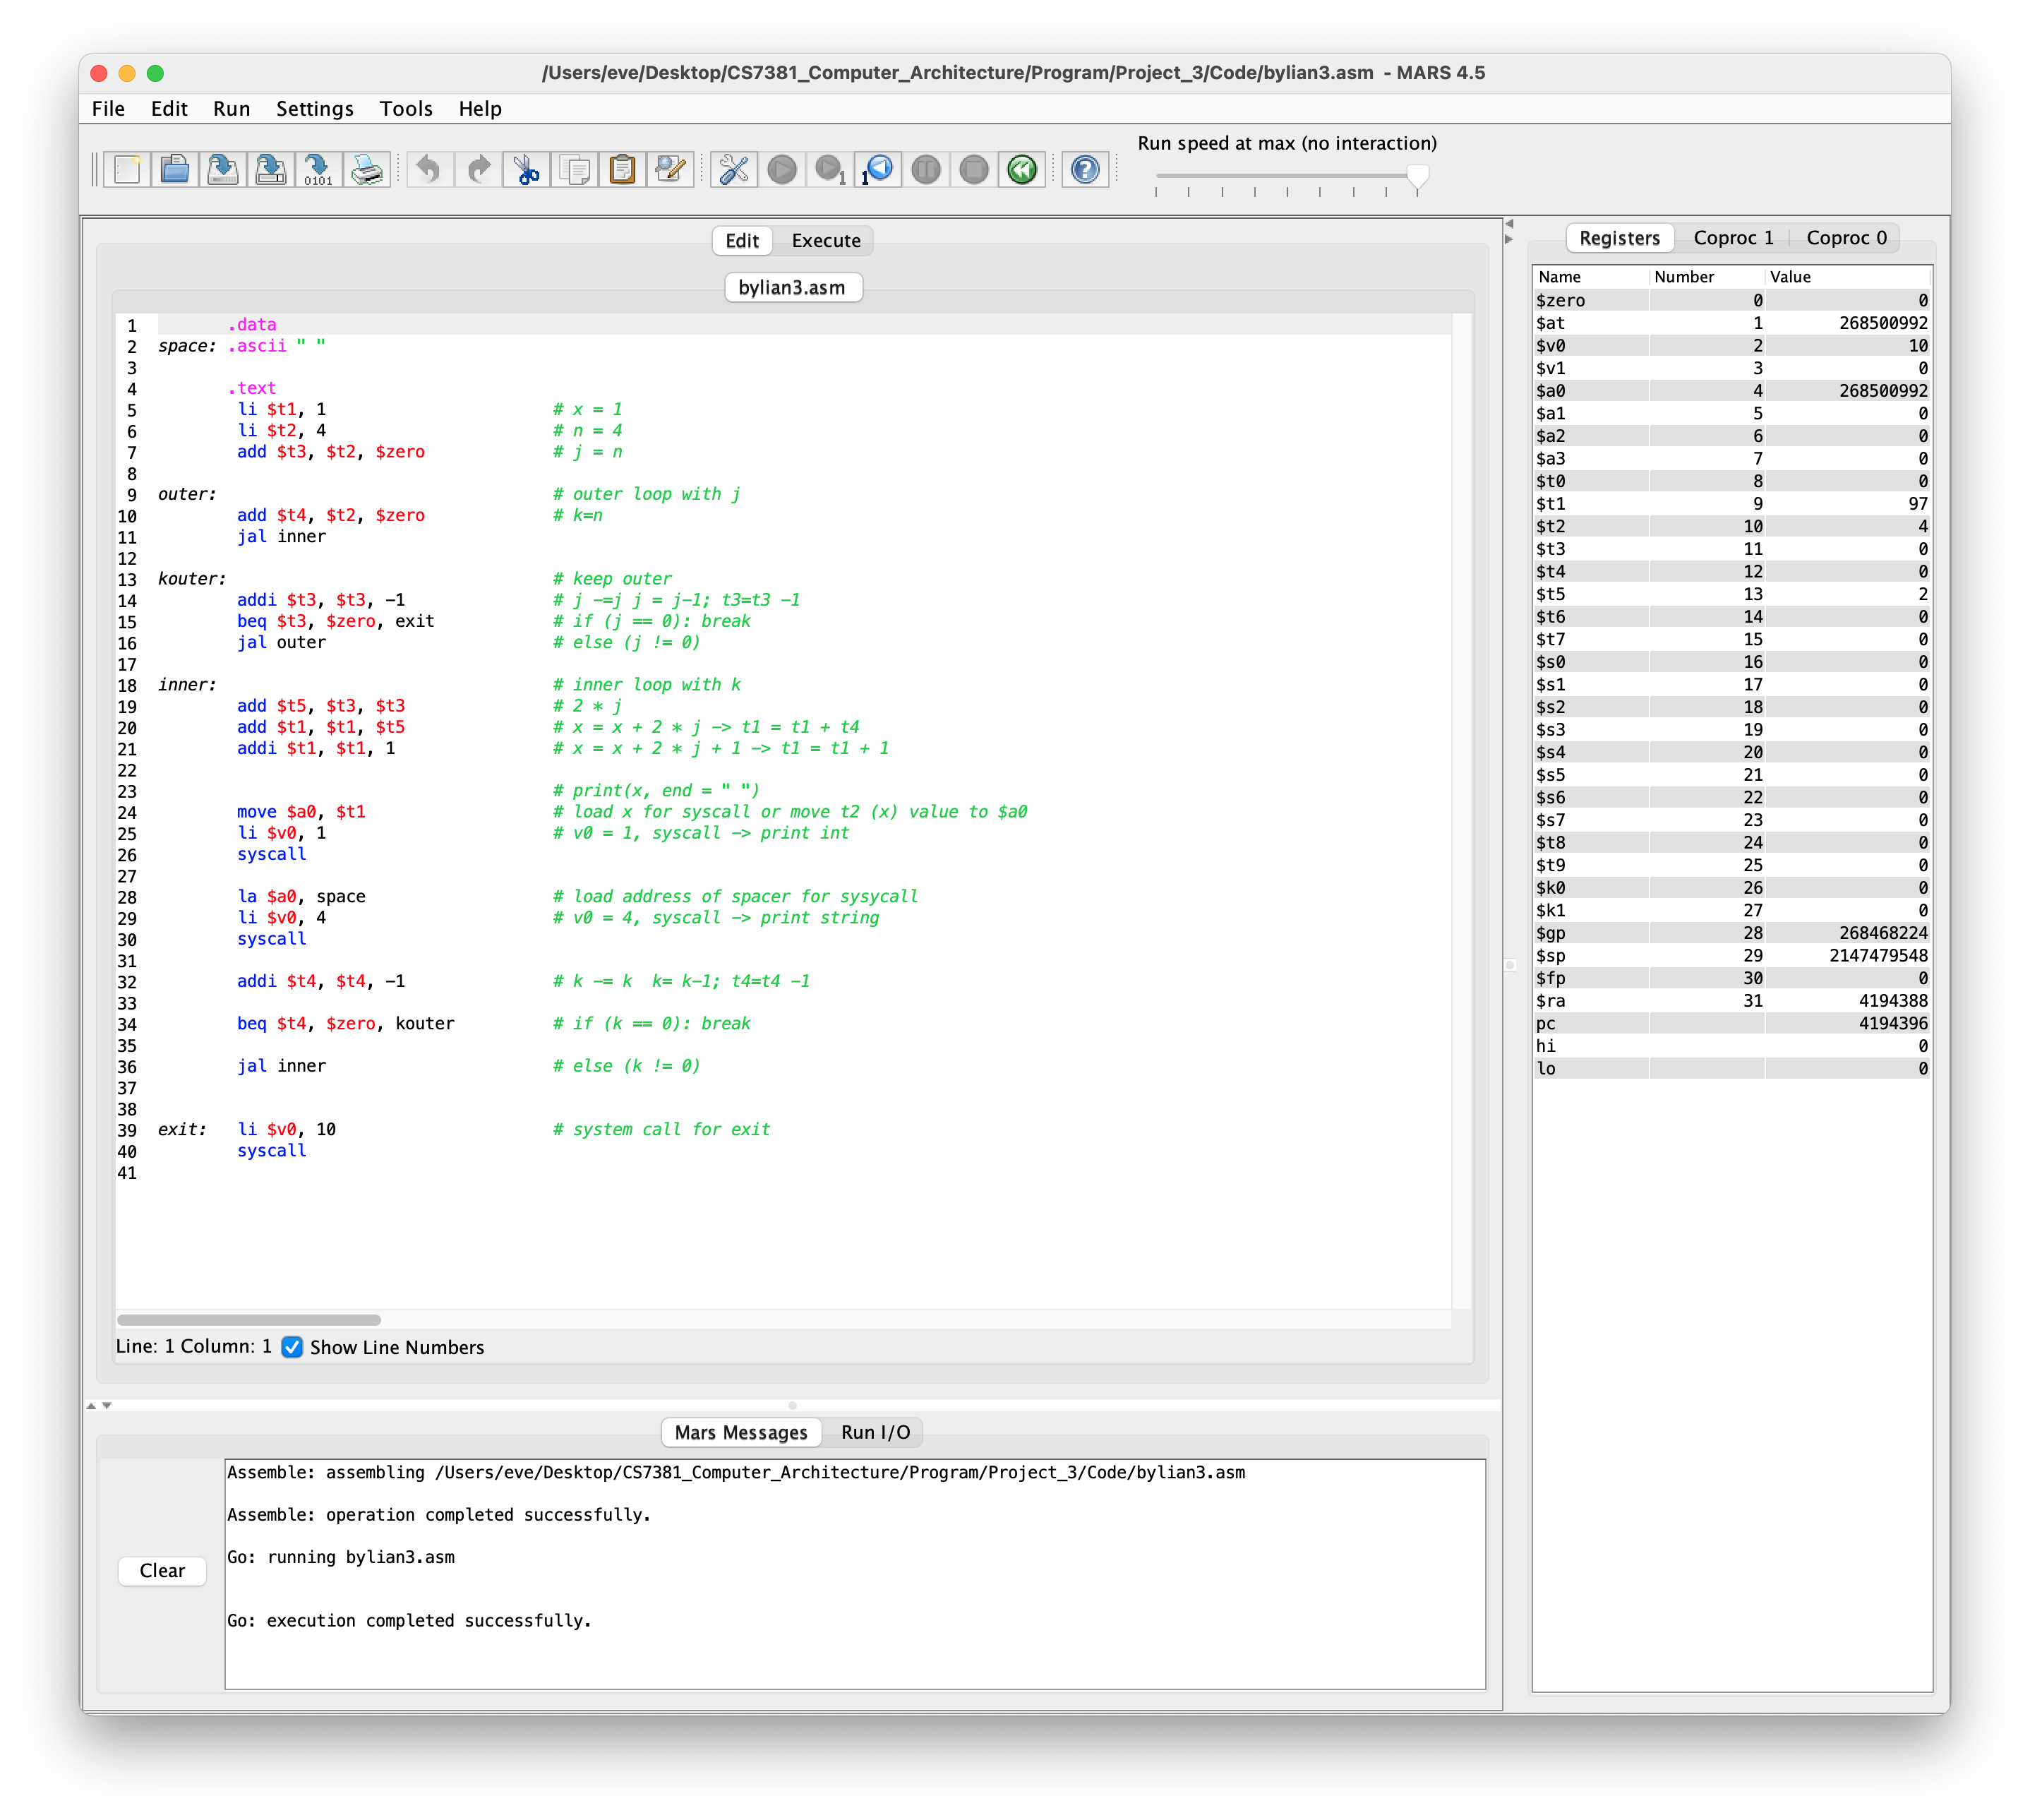
\includegraphics[width=1.1\textwidth]{p2.png}
    \end{center}


\end{document}
